\section{Preliminary Investigations}
    \label{Sec:Results_Preliminary}
%! Motivation / Intro
In the following, the feasibility of depositing \cro\ thin films via \gls{pld} as well as their resulting physical properties are investigated.
Because \cro\ is the most stable chromium oxide, its formation is expected, but other oxidation states cannot be excluded.
E.g., in Fig.\,\ref{Fig:Results_2_photoTarget}, a silver colored target coating can be observed, presumably corresponding to metallic \ce{CrO2}.
If \cro\ is the only oxidation state, then amorphous or rhombohedral films are expected, because no other polymorph of \cro\ exists.
Furthermore, if a crystalline phase is present, the orientation with respect to the sapphire substrates is of interest.
Because \alo\ and \cro\ exhibit the same crystal symmetry, it is expected that the crystal orientation of the film  matches the corresponding substrate orientation.
Finally, deposition parameters should be optimized to obtain the best crystal quality.

\subsection{Experiment}
    Due to the similar crystal structure of \cro\ and \agao, the deposition parameters of the latter were chosen as a starting point to deposit chromia thin films on $10\times\qty{10}{\mm\squared}$ sapphire substrates with \textit{m}-plane orientation.
Namely, a pulse energy of \qty{650}{mJ} and a pulse frequency of \qty{20}{\Hz} were applied for a total of \qty{30000} pulses.
To investigate the influence of deposition parameters, three batches were produced:
\begin{enumerate}
    \item variation of oxygen partial pressure from \qtyrange{8e-5}{1e-2}{mbar} with a fixed temperature of \qty{745}{\degreeCelsius},
    \item variation of growth temperature from \qtyrange{725}{765}{\degreeCelsius} with a fixed oxygen partial pressure of \qty{1e-3}{mbar}, and
    \item variation of substrate orientation between \textit{c}- (00.1), \textit{r}- (01.2) \textit{m}- (10.0) and \textit{a}-plane (11.0) $5\times\qty{5}{\mm\squared}$ sapphire substrates\footnote{
        In the following, the \textsc{Bravais}-\textsc{Miller}-indices will be omitted.
        }
    with a fixed oxygen partial pressure of \qty{1e-3}{mbar} and a growth temperature of \qty{715}{\degreeCelsius}.
\end{enumerate}
Structural properties of those thin films were determined by \thetaomega-scans, \textomega-scans and \textphi-scans.
The thickness was determined via spectroscopic ellipsometry, and transmission spectra were recorded for two samples of the 1st batch to determine the optical band gap.
Temperature dependent resistivity measurements were performed on the samples of the 3rd batch.

% \subsection{Results}
    \subsection{Oxygen Partial Pressure Variation on \textit{m}-plane Sapphire}
        %! 2theta-omega scans
\begin{figure}
    \centering
    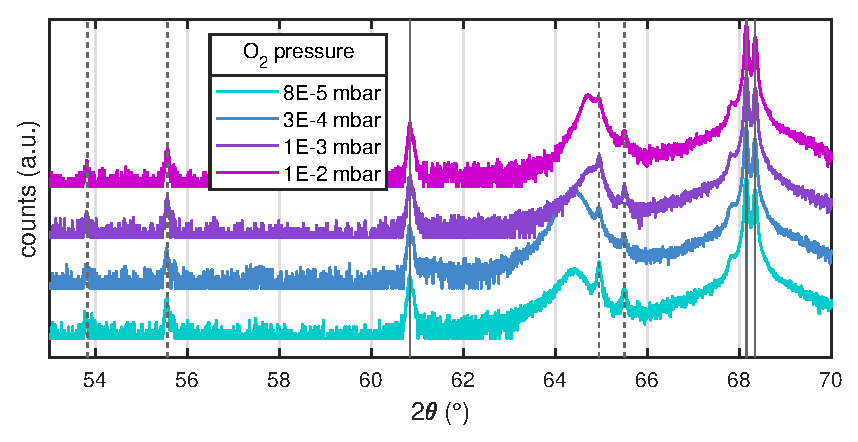
\includegraphics{1_pressure_2theta.eps}
    \caption{\thetaomega-patterns of \cro\ thin films deposited on \textit{m}-plane sapphire for various oxygen partial pressures.
    The solid lines indicate (30.0) substrate reflections corresponding to copper radiation, whereas the dashed lines indicate (30.0) substrate reflections corresponding to tungsten radiation.}
    \label{Fig:Results_1_pressure_2theta}
\end{figure}
In the following, the results for the samples produced at four different oxygen partial pressures are analyzed.
In Fig.\,\ref{Fig:Results_1_pressure_2theta}, the \thetaomega-patterns are depicted.
For each pattern, the two peaks (solid line) at around \qty{68}{\degree} correspond to the (30.0) reflection of the \textit{m}-plane oriented sapphire substrate.
The splitting occurs due to the similar wavelength of \ce{Cu}-K\textalpha\textsubscript{1} and \ce{Cu}-K\textalpha\textsubscript{2} radiation.
The additional peaks also stem mainly from the (30.0) reflection of \ce{Al2O3} and are caused by
\ce{W}-L\textbeta\textsubscript{2}-,
\ce{W}-L\textbeta\textsubscript{1}-,
\ce{Cu}-K\textbeta-,
\ce{W}-L\textalpha\textsubscript{1}- and
\ce{W}-L\textalpha\textsubscript{2}-radiation (increasing angles).\footnote{
    %TODO
    \bfseries\textcolor{red}{Klar wäre das besser das im plot an die linien zu schreiben, aber das war mir irgendwie zu auffändig es schön zu machen. Gehts auch so?}
}
In the vicinity of the calculated peak position for the (30.0) reflection of \cro\ (cf.~\ref{tab:d_strained}), there is a peak observed for each sample, indicating that the \textalpha-phase of \cro\ is present.
Note that the peak position is varying depending on the chosen oxygen partial pressure.
The difference to the expected peak position $2\theta_0$ is expressed as \gls{oop}\ strain $\epsilon_{zz}$ using the Bragg equation \eqref{Equ:Theory_BraggCondition} and then
\begin{equation}
    \label{Equ:Results_oop_strain_def}
    \epsilon_{zz}
    =\frac{d-d_0}{d_0}
    =\left(\frac{1}{\sin(2\theta/2)}-\frac{1}{\sin(2\theta_0/2)}\right)
    \cdot\sin(2\theta_0/2)\,.
\end{equation}
In Fig.\,\ref{Fig:Results_1_both_strainFWHM}a, the calculated strain is shown in dependence of the corresponding oxygen partial pressure.
The strain decreases from approx.\ \qty{0.95}{\percent} to \qty{0.45}{\percent} with increasing pressure.
This strain reduction may therefore be the result of increased background gas scattering which results in less kinetic energy of the specimen reaching the heated substrate (cf.~\ref{Sec:Methods_pld}).
\begin{figure}
    \centering
    \begin{tabular}{ll}
        \textbf{(a)}&\textbf{(b)} \figSpace\\
        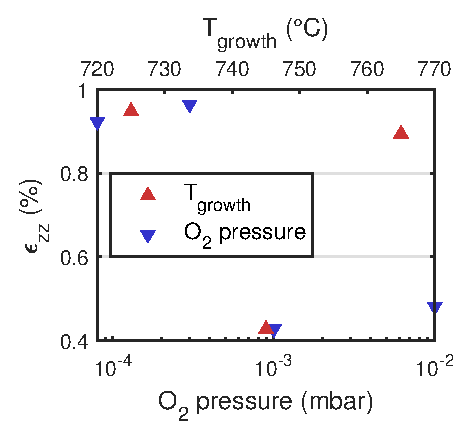
\includegraphics[align=c]{1_both_strain.eps}    
        &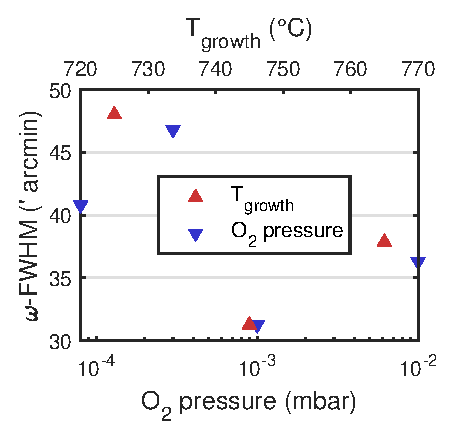
\includegraphics[align=c]{1_both_FWHM.eps}
    \end{tabular}
    \caption{
        \textbf{(a)} \gls{oop}\ strain calculated with \eqref{Equ:Results_oop_strain_def} and \textbf{(b)} \textomega-FWHMs for samples from growth temperature series (red triangles, top \textit{x}-axis) and oxygen partial pressure series (blue triangles, bottom \textit{x}-axis).
        }
    \label{Fig:Results_1_both_strainFWHM}
\end{figure}

%! omega-scans
For each sample, the $2\theta$ angle was fixed to the observed (30.0) reflection of \cro\ and an \textomega-scan was performed.
The \gls{FWHM} of the \textomega-patterns (henceforth \enquote{\textomega-FWHM}) are depicted in
    Fig.\,\ref{Fig:Results_1_both_strainFWHM}b.
The values vary between approx.\ \qtylist{30;50}{\arcminute} and show a dependence on oxygen partial pressure, which is less pronounced compared with \gls{oop}\ strain
    (Fig.\,\ref{Fig:Results_1_both_strainFWHM}a).
Still, since \textomega-FWHM is connected to the mosaicity of the thin film, higher oxygen partial pressures yield slightly better crystal qualities.
Note that due to the fact that an oxygen partial pressure of \qty{1e-3}{\milli\bar} yielded the best crystal quality, this value is used for future deposition processes.

%! phi-scan
To probe for rotational domains of the thin films, \textphi-scans were performed by fixing $2\theta$ and $\omega$ to the corresponding angles of the (30.6) plane of \cro, which has an inclination angle of \qty{32.4}{\degree} with respect to the (30.0) plane.
The diffraction patterns are depicted in Fig.\,\ref{Fig:Results_1_phiScan}.
The observed peaks of the thin film align with the peaks of the single crystal substrate, indicating that the film has no in-plane rotation with respect to the substrate.
Furthermore, the absence of additional peaks indicates that there exists only a single domain of the thin film\footnote{
    %TODO
    \textcolor{red}{\nopagebreak Vielleicht müsste ich noch erwähnen warum die beiden Reflections hier bei +55° und -55° liegen, also 110° auseinander.
    Aber das versteh ich selber nicht so richtig :( ich würde erwarten dass sie 180° auseinander liegen.}
}.
\begin{figure}
    \centering
    \includegraphics{1_both_phi.eps}
    \caption{Diffraction patterns of \textphi-scans performed on the inclined (30.6) reflections for \textit{m}-plane \cro\ (darker color) and \ce{Al2O3} (brighter color).
    The diffraction patterns cover the samples from variation of oxygen partial pressure (teal to blue colored) and variation of growth temperature (red to yellow colored).
    }
    \label{Fig:Results_1_phiScan}
\end{figure}

%! growth rates
The growth rate $g$ varies between \qtylist{3;7}{\pm\per\pulse} and is depicted in Fig.\,\ref{Fig:Results_1_growthRates_photograph}a.
No systematic dependence on the oxygen partial pressure can be observed.
\begin{figure}
    \centering
    \begin{tabular}{ll}
        \textbf{(a)} & \textbf{(b)} \figSpace\\
        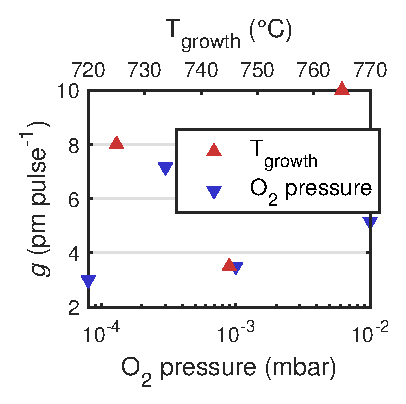
\includegraphics[align=c]{1_both_growthrate.eps}
        &\includegraphics[align=c]{camera_initial.eps}
    \end{tabular}
    \caption{
        \textbf{(a)} Growth rates $g$ for samples from growth temperature series (red triangles, top \textit{x}-axis) and oxygen partial pressure series (blue triangles, bottom \textit{x}-axis).
        \textbf{(b)} Image of the samples produced at different oxygen partial pressures and different growth temperatures.
        }
    \label{Fig:Results_1_growthRates_photograph}
\end{figure}

%! Transmission
The transmission spectra of two selected \cro\ thin films are shown in Fig.\,\ref{Fig:Results_1_transmission}a.
The samples are not fully transparent in the visible spectrum and they exhibit a greenish tint, as can also be seen in Fig.\,\ref{Fig:Results_1_growthRates_photograph}b.
% fitting with indirect gap: cheng 1996, al-kuhaili2007 (^1/2)
% fitting with direct gap: farrell 2015 (^2)
% mi2018 states cr2o3 is a direct bandgap semiconductor
To determine the onset of absorption $E_\mathrm{opt}$, an $\alpha^2$ vs.\ $E$ plot (Fig.\,\ref{Fig:Results_1_transmission}b) is utilized (cf.~\ref{Sec:Methods_transmission}).
Although the publications used for reference in this work support the direct transition nature of \cro\ 
    \cite{farrell2015,mi2018},
it has to be noted that there exist studies determining the optical band gap of \cro\ by assuming an indirect transition nature 
    \cite{cheng1996,al-kuhaili2007}.
However, all of them utilize a \textsc{Tauc} plot $(\alpha E)^\eta$ vs.\ $E$, which is an unappropriate method for crystalline solids as discussed in~\ref{Sec:Methods_transmission}.
Therefore, the method based on the assumption of parabolic shape of bands as well as direct transitions (cf.\ \ref{Sec:Methods_transmission}) is used.
Fitting the linear regime in the onset of absorption results in $E_\mathrm{opt}\approx\qty{3.6}{\eV}$ for both samples, which differ in strain and \textomega-FWHM by a factor of approx.\ 2 and 0.3, respectively.
\begin{figure}
    \centering
    \begin{tabular}{c}
        \multicolumn{1}{l}{\textbf{(a)}}\figSpace\\
        \includegraphics[align=t]{1_pressure_transmission.pdf}\figSpace\\
        \multicolumn{1}{l}{\textbf{(b)}}\figSpace\\
        \includegraphics[align=t]{1_pressure_tauc.pdf}
    \end{tabular}
    \caption{\textbf{(a)} Transmission spectra of two selected \cro\ thin films, deposited with different oxygen partial pressures. The spectra are normalized to a corresponding uncoated \textit{m}-plane sapphire substrate.
    \textbf{(b)} $\alpha^2$ vs.\ $E$ plot of the above-mentioned samples.
    It is assumed that \cro\ has a direct bandgap
        \cite{farrell2015,mi2018}.
    The fitting regime is chosen to be between \qtylist{3.75;4.3}{\eV}.
    }
    \label{Fig:Results_1_transmission}
\end{figure}
    \subsection{Growth Temperature Variation on \textit{m}-plane Sapphire}
        In the following, the results for the three samples produced at different growth temperatures are presented.
In addition to the oxygen partial pressure, the influence of growth temperature is investigated.  
%! 2theta-omega
Similar to the previous results, the (30.0) reflection of the \textalpha-phase of \cro\ can be observed (Fig.\,\ref{Fig:Results_1_temperature_2theta}).
% Note that the additional peaks are corresponding to the (30.0) reflection of the substrate and stem from various radiation wavelengths.
The calculated \gls{oop}\ strain is shown in Fig.\,\ref{Fig:Results_1_pressureTemperature_yyaxis_strainOmega}b and a large spread of strain can be observed, varying between \qtylist{0.4;1}{\percent}.
Note that there is no systematic dependence on growth temperature.
\begin{figure}
    \centering
    \includegraphics{1_temperature_2theta_labelled.pdf}
    \caption{
        \thetaomega-pattern of \cro\ thin films deposited on \textit{m}-plane sapphire for three different growth temperatures.
        The gray solid lines indicate (30.0) substrate reflections corresponding to copper radiation, whereas the gray dashed lines indicate (30.0) substrate reflections corresponding to tungsten radiation.
        The red line corresponds to the predicted (30.0) reflection of \cro.
    }
    \label{Fig:Results_1_temperature_2theta}
\end{figure}
%! omega
The \textomega-FWHMs of the \cro\ (30.0) reflection are shown in Fig.\,\ref{Fig:Results_1_pressureTemperature_yyaxis_strainOmega}b and exhibit a similar spread as the samples with varying oxygen partial pressure, but similar to the \gls{oop}\ strain, no dependence on growth temperature is observed.
%! phi-scan
The \textphi-scans (Fig.\,\ref{Fig:Results_1_phiScan}) show that the thin films are in-plane aligned with the respective substrate and that no rotational domains are present.
%! growth rate
Finally, the growth rate varies between \qtylist{3.5;10}{\pm\per\pulse} with no observable dependence on growth temperature.
    \subsection{Influence of Growth Rate on Crystal Structure}
        %! Why is there another explanation needed?
It has to be noted that there is a large spread in strain, \textomega-FWHM and growth rate for the samples that were deposited at different growth temperatures.
The range of temperature variation was only \qty{40}{\degreeCelsius} and has no significant influence on the distribution of strain and \textomega-FWHM (Fig.\,\ref{Fig:Results_1_pressureTemperature_yyaxis_strainOmega}b).
Note that for the last two samples produced with heater temperatures of $T=\qty{725}{\degreeCelsius}$ and $T=\qty{765}{\degreeCelsius}$, respectively, the pulse number was increased to \qty{40000}{pulses}, leading to thicker samples.
But the crystal structure does not depend on thickness either (not shown).
Because all the other process parameters were kept the same, this indicates that another parameter influences the crystal quality.
This is supported by the fact that the growth rate correlates with the magnitude of strain and \textomega-FWHM, as can be seen in Fig.\,\ref{Fig:Results_1_growthRate_process}a (the outlier with low growth rate but high strain will be explained below).
Note that at this point, the growth rate cannot be deconvoluted from the thin film thickness.
Therefore, it is not clear whether the thickness or the reduced growth rate influences the crystal quality.
% Although strain is related to \textomega-FWHM, it has to be noted that for a small regime of \gls{oop}\ strain around approx.\ \qty{0.9}{\percent}, the \textomega-FWHM scatters between approx.\ \qty{37}{\arcminute} and \qty{47}{\arcminute}.

%! importance of process order
The origin of the varying growth rate -- and therefore varying crystal quality -- can be found when taking the number of processes into account that were performed before a specific process.
In Fig.\,\ref{Fig:Results_1_growthRate_process}b, the growth rate is visualized depending on the order of sample fabrication.
It is also indicated when, the laser entrance window has been cleaned.
It is common practice to clean the latter every couple of processes due to coating with target material which absorbs laser energy.
E.g., in the case of \ce{ZnO}, even after \qty{100000}{pulses}, no significant influence can be observed on the transmission of laser energy.
But from Fig.\,\ref{Fig:Results_1_growthRate_process}b it becomes clear that this should be done much more frequently when working with \cro.
Note that the laser has a wavelength of \qty{248}{\nm}, corresponding to \qty{5.0}{\eV}, which is not transmitted by \cro\ thin films\footnote{
    To be precise, the transmission spectrum in Fig.\,\ref{Fig:Results_1_transmission}a is recorded for \textit{m}-plane oriented \textit{crystalline} \cro\ thin films. This may not be the present phase when \cro\ deposits on the (colder) window made out of glass, where it may form an amorphous phase.
},
as can be seen in Fig.\,\ref{Fig:Results_1_transmission}a.
Therefore, the increasing coating of the laser entrance window with each new process absorbs a large amount of laser pulse energy, resulting in less fluence on the PLD target.
This results in less ablated target material and less kinetic energy of the ablated species, which leads to a reduced growth rate and different crystal growth conditions that have less strain and \textomega-FWHM as a result.
\begin{figure}
    \centering
    \begin{tabular}{ll}
        \textbf{(a)} & \textbf{(b)} \figSpace\\
        \includegraphics[align=c]{1_initial_strainOmegaCorrelation.eps}
        &\includegraphics[align=c]{1_initial_window.eps}
    \end{tabular}
    \caption{
        \textbf{(a)} Correlation of \textomega-FWHM with \gls{oop}\ strain, as well as correlation of both with growth rate $g$ (false color).
        The dashed line is a linear fit serving as guide to the eye.
        The outlier with low growth rate but large strain can be explained by accounting for the low oxygen partial pressure of \qty{8e-5}{\milli\bar} for this sample.
        This results in larger kinetic energy of the plasma species.
        \textbf{(b)}~ Growth rate depending on order of sample fabrication.
    }
    \label{Fig:Results_1_growthRate_process}
\end{figure}

%! compatable with oxygen explanation
This explanation is supported by the dependence of crystal quality on oxygen partial pressure (cf.\ Fig.\,\ref{Fig:Results_1_pressureTemperature_yyaxis_strainOmega}a).
There, the increasing crystal quality with higher oxygen pressures is attributed to the increased background gas scattering resulting in less kinetic energy of the plasma material.
This also explains the outlier in Fig.\,\ref{Fig:Results_1_growthRate_process}a, where one sample corresponds to a higher strain and \textomega-FWHM of approx.\ \qty{0.9}{\percent} and \qty{41}{\arcminute}, respectively (black square).
This is not expected when considering the rather small growth rate of \qty{3}{\pm\per\pulse} (\texttt{W6724} in Fig.\,\ref{Fig:Results_1_growthRate_process}b).
But when taking into account that this sample is fabricated at a very low oxygen partial pressure of \qty{8e-5}{\milli\bar}, it becomes clear that although the reduced fluence on the target would generally lower the kinetic energy of the plasma material, the limited scattering with the background gas counteracts this effect, resulting in the observed crystal quality.

%! phi-dependence of strain
It is noteworthy that the observed strain (cf.\ Fig.\,\ref{Fig:Results_1_pressureTemperature_yyaxis_strainOmega}a,b) is distributed around two distinct values of approx.\ \qty{0.4}{\percent} and \qty{0.9}{\percent}.
A prior reported thin film tilt for \textit{m}-plane oriented rhombohedral heterostructures
    \cite{kneiss2021}
may be the reason for this observation:
the samples are installed in the XRD device in such a way that the \textit{c}-axis is either parallel or orthogonal to the scattering plane.
This orientation is arbitrary, and thus the (expected) thin film tilt is either along the X-ray beam or perpendicular to it, which could result in unexpected results when calculating the \gls{oop}\ lattice plane distance from the observed peak position.
To check if this is the origin of the observed strain, for two samples of different strain according to Fig.\,\ref{Fig:Results_1_pressureTemperature_yyaxis_strainOmega}, four \thetaomega-scans were performed with incrementing the azimuth by \qty{90}{\degree} after each measurement.
The resulting diffraction patterns are depicited in Fig.\,\ref{Fig:Results_1_checkPhi}.
The strain is independent of azimuth, only the peak intensity is altered by the in-plane rotation of the sample as expected.
For both samples, an azimuth of \qtylist{0;180}{\degree} results in a lower intensity, supporting the hypothesis that the (expected) thin film tilt is perpendicular to scattering plane which results in a deviation from the \gls{bc}.
Therefore, the distribution of observed strain is not a measurement artifact.
\begin{figure}
    \centering
    \includegraphics{1_initial_checkPhiDependence.eps}
    \caption{
        \thetaomega-patterns for two samples in four different azimuths each.
        The black dashed line indicates the expected (30.0) reflection of \cro.
        }
    \label{Fig:Results_1_checkPhi}
\end{figure}

    \subsection{Deposition on \textit{c}-, \textit{r}-, \textit{m}- and \textit{a}-plane Sapphire}
        %! theta-omega
For the samples deposited on substrates with different orientation, \thetaomega-patterns were recorded (Fig.\,\ref{Fig:Results_1_w6788_2theta}).
For each sample, the expected substrate peaks are observed:
(00.6) and (00.12) for \textit{c}-plane;
(01.2), (02.4), (03.6) and (04.8) for \textit{r}-plane;
(30.0) for \textit{m}-plane;
(11.0) and (22.0) for \textit{a}-plane.
Several smaller peaks also correspond to those reflections but stem from other X-rays than \ce{Cu}-K\textalpha\ (cf.\ Fig.\,\ref{Fig:Results_1_pressure_2theta}).
The mentioned reflections are also observed for the \cro\ thin film, but with a shift in $2\theta$ position similar to the previously investigated \textit{m}-plane samples (Tab.\,\ref{Tab:Results_1_w6788}).
Note that for \textit{r}-plane, the higher order reflections of \cro\ cannot be observed.
It can be concluded that \cro\ grows in the \textalpha-phase on sapphire substrates of different orientation, where the thin film orientation matches the corresponding substrate.
Henceforth, \enquote{\textit{c}-plane \cro} will refer to a \cro\ thin film deposited on \textit{c}-plane oriented $5\times\qty{5}{\mm\squared}$ sapphire substrates, and so on.
\begin{figure}
    \centering
    \includegraphics{1_W6788_2theta_labeled.eps}
    \caption{\thetaomega-patterns of \cro\ thin films deposited on \textit{c}-, \textit{r}-, \textit{m}- and \textit{a}-plane sapphire.}
    \label{Fig:Results_1_w6788_2theta}
\end{figure}
% consider putting [h] to avoid crashing of table with figure
\begin{table}
    \centering
    \caption{Structural parameters, approximate resistivity at room temperature and activation energy for \cro\ thin films of different orientation.}
    \begin{tabular}{ccccc}
        \toprule
        Plane
            & $\epsilon_{zz}$ (\unit{\percent})
            & \textomega-FWHM (\unit{\arcminute}) 
            & $\rho$ (\unit{\ohm\cm})
            & $E_A$ (\unit{\milli\eV})\\
        \midrule
        \textit{c}  &   1.71    &   42.6    &   3       &   57, 34  \\
        \textit{r}  &   0.72    &   38.4    &   120     &   117     \\
        \textit{m}  &   0.55    &   42.6    &   3600    &   240     \\
        \textit{a}  &   1.41    &   32.4    &   4900    &   259     \\
        \bottomrule
    \end{tabular}
    \label{Tab:Results_1_w6788}
\end{table}
%! Omega-scans
For each sample, \textomega-scans were performed on the (00.6), (02.4), (30.0) and (11.0) reflections for \textit{c}-, \textit{r}-, \textit{m}- and \textit{a}-plane, respectively.
The resulting \textomega-FWHMs are in the range of approx.\ \qty{30}{\arcminute} to \qty{40}{\arcminute} (Tab.\,\ref{Tab:Results_1_w6788}).

%! Resistivity
Because the resistivity of all samples was too high to measure Hall effect, only resistivity measurements (cf.~\ref{Sec:Methods_vanDerPauw}) were performed for several temperatures (Fig.\,\ref{Fig:Results_1_w6788_TdH}).
The resistivity depends strongly on the orientation of the thin film, the resistivities at room temperature are listed in Tab.\,\ref{Tab:Results_1_w6788}.
A difference of more than three orders of magnitude between \textit{c}-plane and \textit{a}-plane samples is observed.
The linear behavior of the \textsc{Arrhenius}-plot\footnote{
    Visualization of $f(T)$ as $f'(\tau)$ with $f'=\log f$ and $\tau=1/T$.
}
indicates a thermally activated mechanism for conductivity, and thus semiconductive behavior.
Note that no further conclusions can be drawn on the conduction mechanisms due to the missing carrier concentration and mobility data.
By assuming a behavior of the form
\begin{equation}
    \rho\propto\exp\left(\frac{E_A}{k_BT}\right)\,,
\end{equation}
with \textsc{Boltzmann} constant $k_B$, an activation energy $E_A$ can be estimated.
Those energies are also listed in Tab.\,\ref{Tab:Results_1_w6788}.
For \textit{c}-plane \cro, two linear regimes can be distinguished, favoring a dependence of the form
\begin{equation}
    \rho\propto a\exp\left(\frac{E_{A,1}}{k_BT}\right)
    +b\exp\left(\frac{E_{A,2}}{k_BT}\right)\,,
\end{equation}
thus two activation energies are determined.
\begin{figure}
    \centering
    \includegraphics{1_W6788_resistivityTempDep.eps}
    \caption{
        Temperature dependent resistivity measurements for samples with different orientations.
    }
    \label{Fig:Results_1_w6788_TdH}
\end{figure}

\subsection{Conclusion}
    \textit{m}-plane \cro\ thin films can be deposited over a wide range of oxygen partial pressure of more than two orders of magnitude.
It turned out that the crystal quality correlates mainly with the growth rate, which is presumably caused by a variation of the laser pulse fluence on the target.
Therefore, lower kinetic energy of the plasma species is probably the reason for improved crystallinity and less strain.
Even though the influence of those parameters was less dominant, an oxygen partial pressure of \qty{1e-3}{\milli\bar} and a heater temperature of \qty{750}{\degreeCelsius} are identified as best growth conditions.
Note that those values overlap with the conditions for deposition \agao, which makes ternary solid solutions of chromia with rhombohedral \gao\ feasible.

\textalpha-\cro\ was also deposited on \textit{c}-, \textit{r}- and \textit{a}-plane sapphire, with the thin films crystallizing in the respective orientation.
This is important for heterostructures with \agao\ and could enable growth of rhombohedral \gao\ on all common sapphire cuts via \cro\ buffer layers.
Note that all deposited thin films showed a discrepancy between observed \gls{oop}\ lattice constants and bulk \cro\ literature values (Tab.\,\ref{Tab:sesquiLatticeConstants}).
The conductivity is strongly dependent on the crystal orientation and was very low for the prismatic orientations, but with \qty{0.3}{\siemens\per\cm} three orders of magnitude higher for the basal orientation.